\subsection*{Quantum Teleportation}
In the teleportation protocol, the two parties (guess who)  share the entangled Bell State and it is implemented via a CNOT gate between the state to be sent (suppose Alice is sending the state) and the part of entangled Bell state Alice has. The CNOT gate creates another entangled state whose measurement Alice will send to the second party, say it's Bob, to perform the measurements accordingly. So if you assume the state to be sent is 1 qubit state after CNOT you will have a 3 qubit state (as Bell sate is 2 qubit state). Now Alice will measure the middle qubit which will be the part of classical information she will communicate to Bob.

So, you see the controlled-NOT acts as an entangling operator without affecting the first qubit (here $\ket{\psi}$) and changing the entangled Bell state and hence its measurement outcome.
A general description of this cool phenomena is shown in figure: 
\begin{figure}[h!]
    \centering
    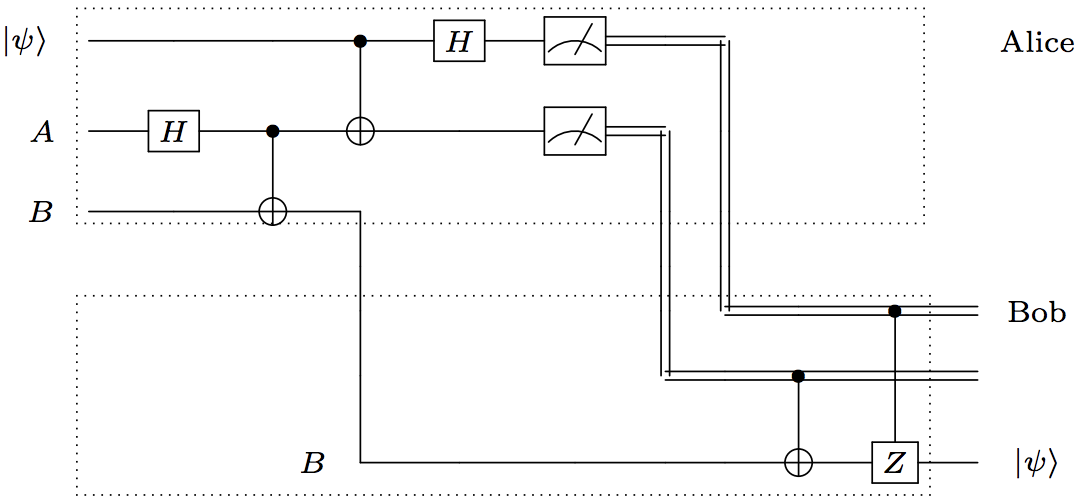
\includegraphics[width=\textwidth]{Mainmatter/images/teleportation-circuit.png}
    \caption{Basic circuit which implements quantum teleportation}
    \label{fig:teleportation}
\end{figure}
Quantum teleportation is very useful in quantum communication because it allows to send classical reliable bits instead of a qubit.